% !TeX encoding = UTF-8
% !TeX program = pdflatex
% !TeX spellcheck = en_US
% !TeX root = paper.tex


\pdfcompresslevel=0
\pdfobjcompresslevel=0

\usepackage[utf8]{inputenc}
\usepackage[T1]{fontenc}
\usepackage{textcomp}
\usepackage{gensymb}
\DeclareUnicodeCharacter{00B0}{\degree}

\usepackage[dvipsnames]{xcolor}
%\usepackage[authoryear,longnamesfirst]{natbib}
\usepackage{amssymb}
%Please add the following packages if necessary:
\usepackage{booktabs, multirow} % for borders and merged ranges
\usepackage{soul}% for underlines

\usepackage{changepage,threeparttable} % for wide tables

%% The lineno packages adds line numbers. Start line numbering with
%% \begin{linenumbers}, end it with \end{linenumbers}. Or switch it on
%% for the whole article with \linenumbers.
\usepackage{lineno}

\usepackage{framed} % Framing content
\usepackage{multicol} % Multiple columns environment

\usepackage[textwidth=3cm, colorinlistoftodos]{todonotes}
\setuptodonotes{fancyline, color=red!15, size=\footnotesize}

\newcommand{\rewrite}[1]{\todo[color=green!40]{#1}}
\newcommand{\addref}{\todo[color=red!40]{Add reference.}}
%\newcommand{\todoo}[2][]{\todo[inline,color=red, #1]{#2}}
\newcommand{\todoo}[2][]{\todo[inline, #1]{#2}}



\usepackage[breaklinks, hidelinks,hyperfootnotes=false, unicode]{hyperref} %Clickable hyperlinks everywhere
\def\UrlBigBreaks{\do\/\do-\do:}
\hypersetup{
	draft=false,
	%    bookmarks=true,
	bookmarksopen=true,
	bookmarksopenlevel=1,  %hier darf nur ne Zahl stehen, ansonsten produziert TeX nen Fehler in Zusammenhang mit 		bookmarksopen
	bookmarksdepth=4, %deprecated
	bookmarksnumbered=true,
	linktocpage=true,       %break links correctly in listoftables/figures
	unicode=true,          % non-Latin characters in Acrobat’s bookmarks
	pdftoolbar=true,        % show Acrobat’s toolbar?
	pdfmenubar=true,        % show Acrobat’s menu?
	pdffitwindow=true,     % window fit to page when opened
	pdfstartview={XYZ null null 1.00},
	%         XYZ 	left top zoom   Sets a coordinate and a zoom factor. If any one is null, the source link value is used. null null null will give the same values as the current page.   Fit   Fits the page to the window.    FitH 	top
	%    Fits the width of the page to the window.    FitV 	left     Fits the height of the page to the window.    FitR 	left bottom right top    Fits the rectangle specified by the four coordinates to the window.    FitB  Fits the page bounding box to the window.
	%    FitBH 	top  Fits the width of the page bounding box to the window.
	%    FitBV 	left  Fits the height of the page bounding box to the window.
	pdftitle = {},    % title
	pdfauthor = {Patrick Kastner},     % author
%	pdfsubject = {Ph.D. Thesis},   % subject of the document
	pdfcreator={Patrick Kastner},   % creator of the document
	pdfproducer={Patrick Kastner}, % producer of the document
%	pdfkeywords= {Computational Fluid dynamics} {Decision-making} {Generative Adversarial Networks} {Outdoor Thermal Comfort} {Ray Tracing} {Urban Design}, % list of keywords
	pdfnewwindow=true,      % links in new window
%	pdfpagelayout={TwoColumnRight},
	colorlinks=false,       % false: boxed links; true: colored links
	linkcolor=black,          % color of internal links
	citecolor=black,        % color of links to bibliography
	filecolor=black,      % color of file links
	urlcolor=black,           % color of external links
	anchorcolor =black,
%	linkbordercolor={blue!35!black},          % color of internal links
%	citebordercolor={blue!35!black},        % color of links to bibliography
%	filebordercolor={blue!35!black},      % color of file links
%	urlbordercolor={blue!35!black},           % color of external links
	menucolor =red,
	runcolor =cyan,
	pdfencoding=auto,
}


% Paragraphs with numbering
%\usepackage{titlesec}
%\setcounter{secnumdepth}{4}
%\titleformat{\paragraph}
%{\normalfont\normalsize\itshape}{\theparagraph.}{1em}{}
%\titlespacing*{\paragraph}
%{0pt}{3.25ex plus 1ex minus .2ex}{1.5ex plus .2ex}

% Paragraphs with semicolon
\usepackage{titlesec}

\setcounter{secnumdepth}{4}
\titleformat{\paragraph}[runin]
{\normalfont\normalsize\itshape}{}{0em}{}[:]
\titlespacing*{\paragraph}
{0pt}{3.25ex plus 1ex minus .2ex}{1em}





%\usepackage{xtab,booktabs}
\usepackage{caption}
% No space under figure
\captionsetup{belowskip=0pt}
\setlength{\belowcaptionskip}{-10pt}

%\usepackage{subcaption}
%\captionsetup[subfloat]{font=sf,size=footnotesize}

\usepackage{float}
\usepackage{sidecap} %captions on the side of figures




\usepackage[acronym, nomain]{glossaries}
\usepackage{glossary-mcols}
\renewcommand{\glsmcols}{2}
\setglossarystyle{mcolindex}
%\renewcommand{\glsnamefont}[1]{\textmd{#1}\mytab} % Regular font for acronyms

%\usepackage{tabto}
%\newcommand\mytab{\tab \hspace{1.4cm}}
%\renewcommand{\glsnamefont}[1]{\textmd{#1}  } % Regular font for acronyms

%\usepackage[]{glossaries-extra}
%\usepackage{glossaries-extra-stylemods}
\makeglossaries

%\setabbreviationstyle[acronym]{short-long}
%\GlsXtrEnableEntryCounting
% {glossaries}% list of categories to use entry counting
% {1}% trigger value (only add to glossary if count > 3)


\usepackage[
separate-uncertainty  = true,
uncertainty-separator =  {\,},
mode = text,
output-decimal-marker ={.},
multi-part-units      = single,
range-units           = single,
%range-phrase          = {--},
]{siunitx} 		%SI Einheit
\sisetup{
	%list-final-separator = { \translate{und} },
	% range-phrase = {\text{~to~}},
	%list-pair-separator = { \translate{und} },
	%exponent-product = \cdot
	detect-all, %apply document fonts for siunitx
	%math-rm=\mathsf,
	%text-rm=\sffamily,
	locale                  = US,
	input-decimal-markers   = {.},
	output-decimal-marker   = {.},
	%input-ignore            = {,},
	%group-digits            = true,
	%group-separator         = {,},
	%group-separator         = {},
	%tight-spacing           = true,
	%input-signs             = ,
	%input-symbols           = ,
	%input-open-uncertainty  = ,
	%input-close-uncertainty = ,
	table-align-text-pre    = false,
        mode=match
}


%\usepackage[final]{pdfpages}
\usepackage{afterpage}

\usepackage{graphbox,graphicx}
\usepackage{pgfplots}
\pgfplotsset{compat=1.18}



\usepackage{cleveref}
\usepackage{nicefrac}


% Remove preprint statement temporarily
\let\today\relax
\makeatletter
\def\ps@pprintTitle{%
    \let\@oddhead\@empty
    \let\@evenhead\@empty
    \def\@oddfoot{\footnotesize\itshape
         {} \hfill\today}%
    \let\@evenfoot\@oddfoot
    }
\makeatother


% Modify vertical space between figure and caption
\setlength{\abovecaptionskip}{5pt plus 3pt minus 2pt} % Chosen fairly arbitrarily
% The default values are 10pt and 0pt. (The plus and minus allows the space to stretch and shrink if needed. The numbers specify how much.)

\journal{Sustainable Cities and Society}

\newacronym{RMSE}{RMSE}{Root Mean Squared Error}


\begin{document}

% \listoftodos
\clearpage

\begin{frontmatter}




\title{My Fancy Title}

     %% Title, authors and addresses


%\author[ESLAB]{Patrick Kastner\corref{mycorrespondingauthor}}
\author[ESLAB]{Patrick Kastner}
%\cortext[mycorrespondingauthor]{Corresponding author}
\ead{pk373@cornell.edu}
%\cormark[1]

\affiliation[ESLAB]{organization={Environmental Systems Lab, Cornell University},
	addressline={252 East Sibley},
	city={Ithaca},
	postcode={14853},
	state={NY},
	country={USA}}

\author[ESLAB]{Timur Dogan}
\ead{tkd9@cornell.edu}
%\ead[url]{https://es.aap.cornell.edu}


%%% Title, authors and addresses
%
%%% use the tnoteref command within \title for footnotes;
%%% use the tnotetext command for theassociated footnote;
%%% use the fnref command within \author or \address for footnotes;
%%% use the fntext command for theassociated footnote;
%%% use the corref command within \author for corresponding author footnotes;
%%% use the cortext command for theassociated footnote;
%%% use the ead command for the email address,
%%% and the form \ead[url] for the home page:
%%% \title{Title\tnoteref{label1}}
%%% \tnotetext[label1]{}
%%% \author{Name\corref{cor1}\fnref{label2}}
%%% \ead{email address}
%%% \ead[url]{home page}
%%% \fntext[label2]{}
%%% \cortext[cor1]{}
%%% \affiliation{organization={},
	%	%%             addressline={},
	%	%%             city={},
	%	%%             postcode={},
	%	%%             state={},
	%	%%             country={}}
%%% \fntext[label3]{}
%
%\title{Title of Your Manuscript}
%
%%% use optional labels to link authors explicitly to addresses:
%%% \author[label1,label2]{}
%%% \affiliation[label1]{organization={},
	%	%%             addressline={},
	%	%%             city={},
	%	%%             postcode={},
	%	%%             state={},
	%	%%             country={}}
%%%
%%% \affiliation[label2]{organization={},
	%	%%             addressline={},
	%	%%             city={},
	%	%%             postcode={},
	%	%%             state={},
	%	%%             country={}}
%
%\author[inst1]{Author One}
%
%\affiliation[inst1]{organization={Department One},%Department and Organization
	%	addressline={Address One}, 
	%	city={City One},
	%	postcode={00000}, 
	%	state={State One},
	%	country={Country One}}
%
%\author[inst2]{Author Two}
%\author[inst1,inst2]{Author Three}
%
%\affiliation[inst2]{organization={Department Two},%Department and Organization
	%	addressline={Address Two}, 
	%	city={City Two},
	%	postcode={22222}, 
	%	state={State Two},
	%	country={Country Two}}

    % Here goes the abstract
    \begin{abstract}
        % Basic Introduction


        % General problem


        % One sentence summarizing the main result (with the words “here we show”)


        % Two or three sentences explaining what the main result reveals in direct comparison to what was previously thought to be the case or how the main result adds to previous knowledge.


        % One or two sentences to put the results into a more general context


        % Two or three sentences to provide a broader perspective, readily comprehensible to a scientist in any discipline


    \end{abstract}

    \begin{graphicalabstract}
        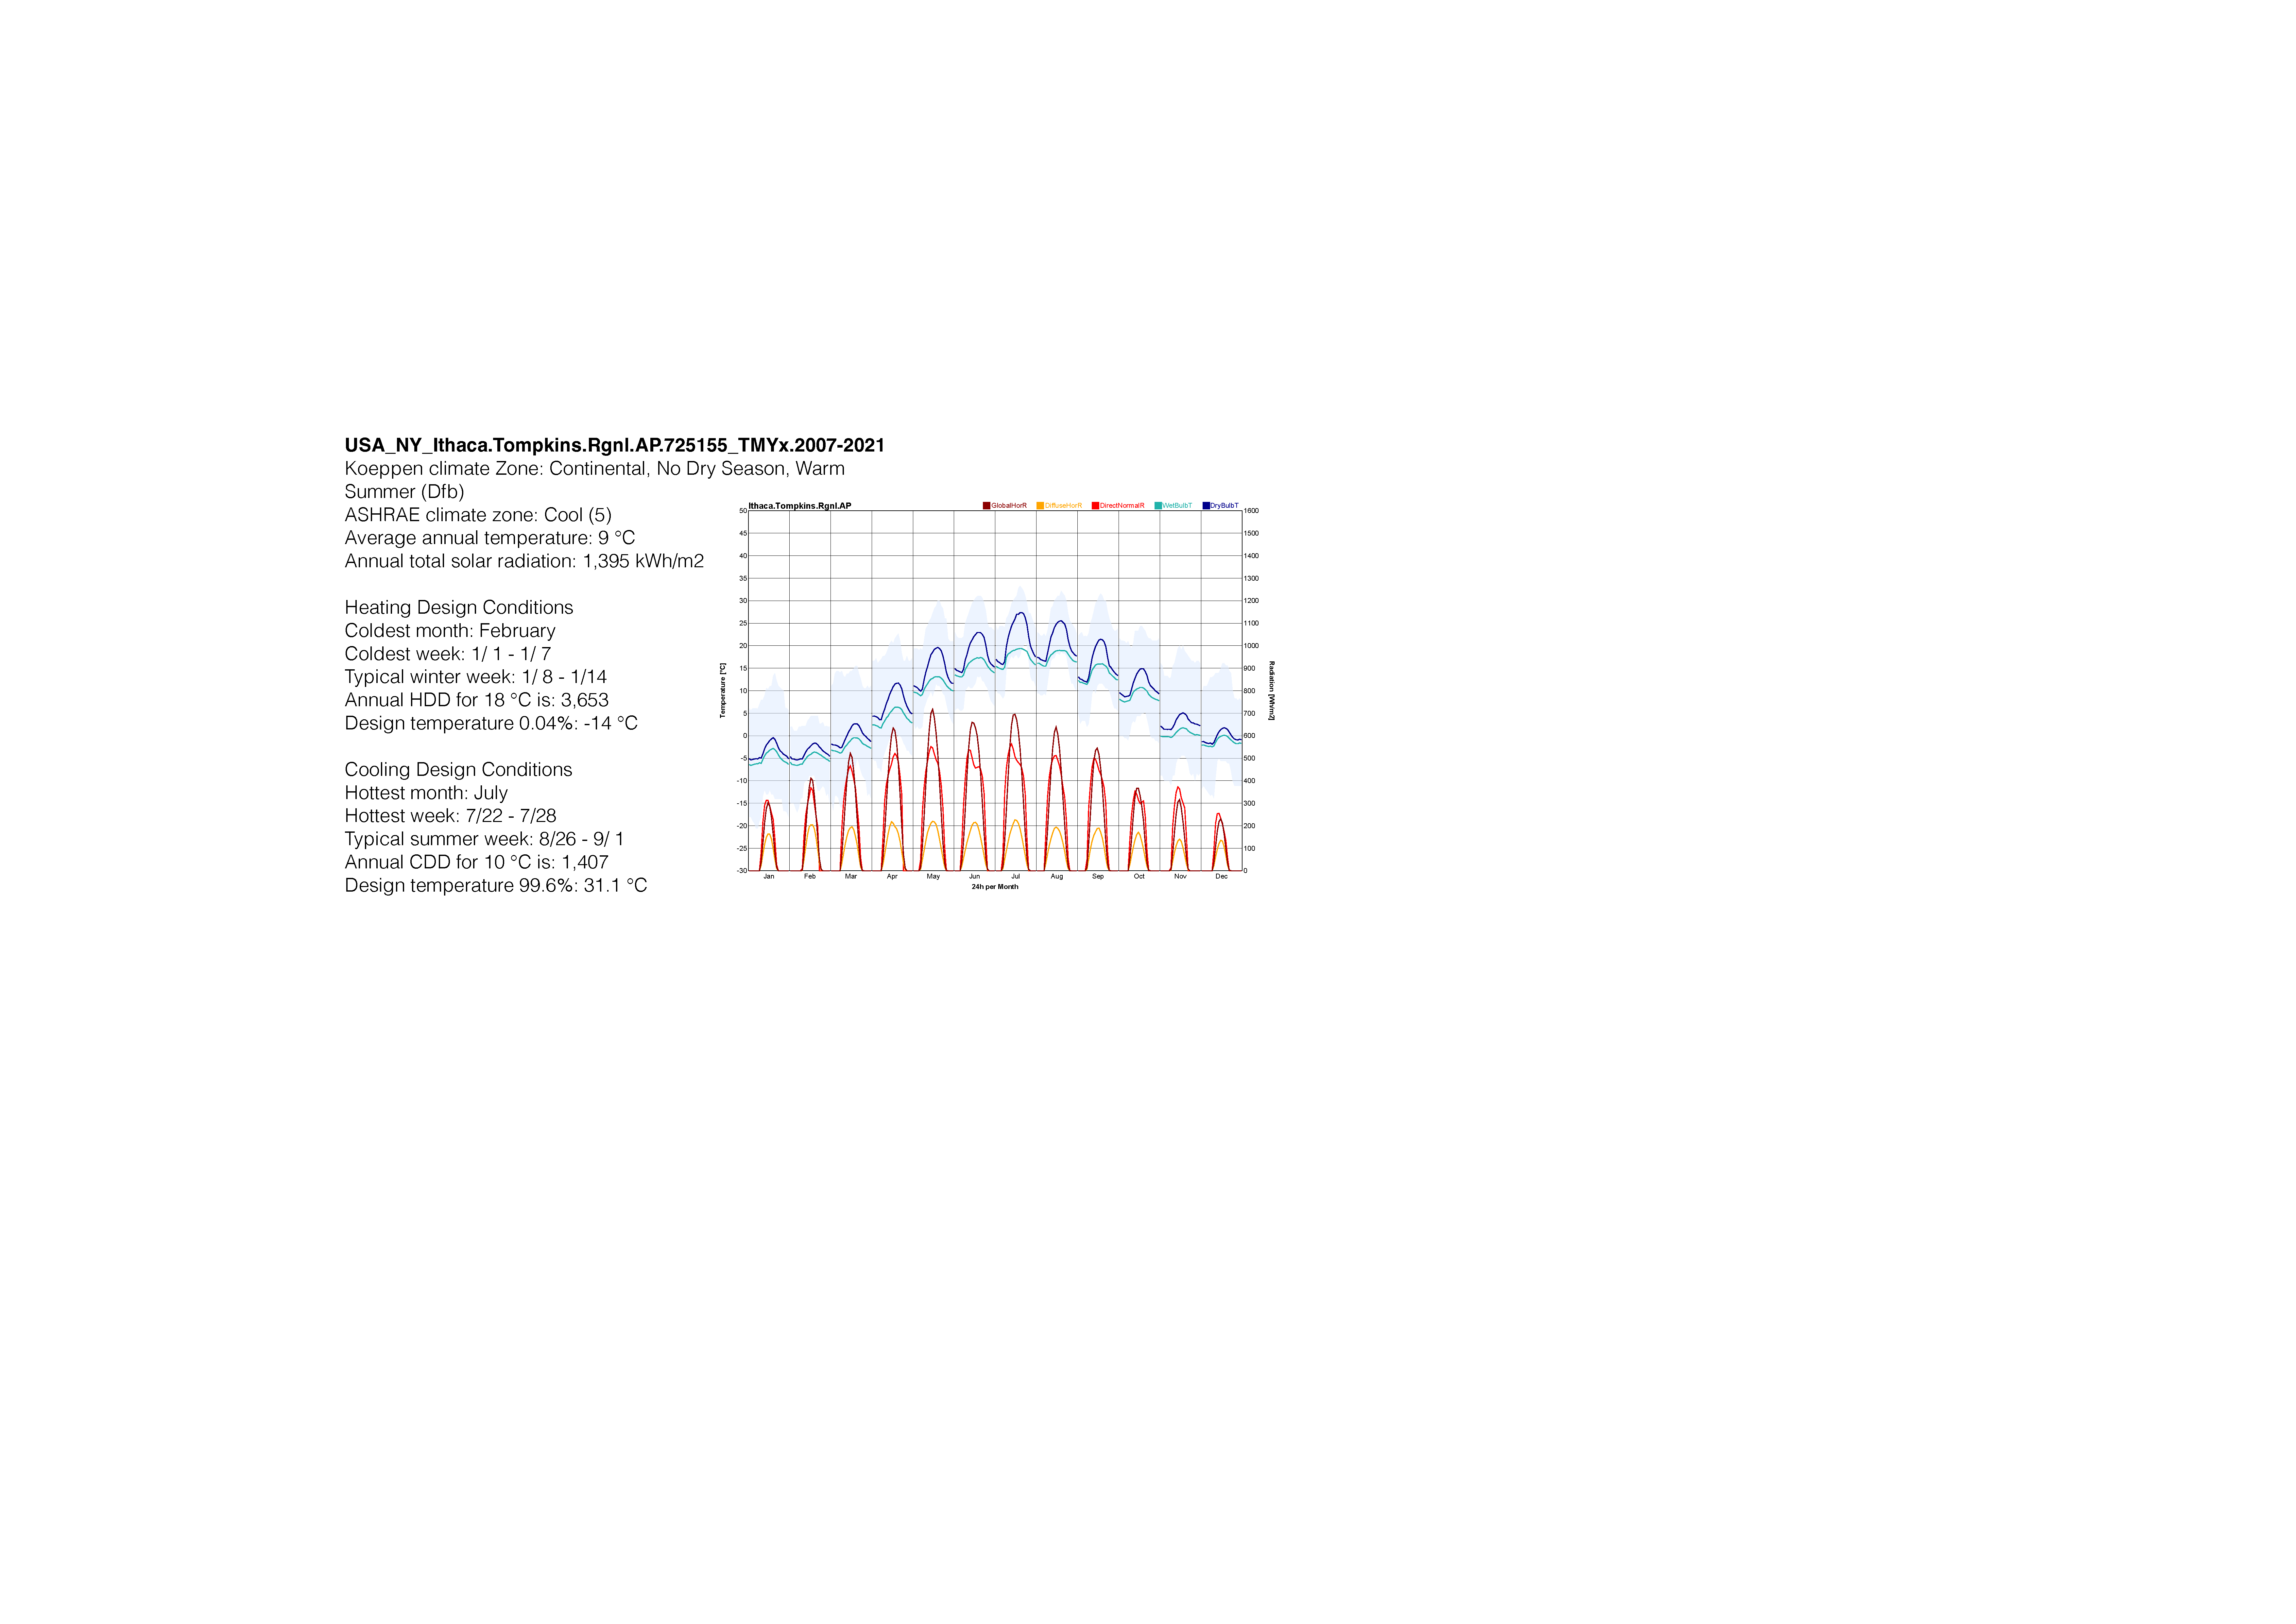
\includegraphics[width=0.9\linewidth]{images/3_IGND}
    \end{graphicalabstract}

    % Research highlights
    \begin{highlights}
		\item 1 %
		\item 2 %
		\item 3 %
    \end{highlights}

    % Keywords separated by \sep
    \begin{keyword}
        Key \sep
        Key \sep
        Key \sep
        Key %\sep
    \end{keyword}

\end{frontmatter}

%\linenumbers
%\modulolinenumbers[5]

\section{Introduction}
\label{sec:Introduction}

% First paragraph: The Hook 1. Sentence starting with what the domain is and why it is important 2. What is the overall problem or situation in that domain
% Second paragraph: The Gap 3. What are the conclusions of existing literature for that problem situation in this domain? 4. What is the problem or issue with that existing literature?
% Third paragraph: The study 5. Indicate how this study addresses that problem or issue 6. Describe the study, sample, and method for addressing that problem or issue
% Fourth paragraph: Contribution and conclusion 7. Describe what you found 8. State explicitly how these findings extend and contribute to existing knowledge
% Fifth paragraph (optional): Outline/roadmap 9. Describe the overall outline of the paper

\subsection{Background and Context}



\subsection{Literature Review}



%\clearpage
%\afterpage{\clearpage}
\section{Methodology}\label{sec:Methodology}



%\afterpage{\clearpage}
%\clearpage
\section{Results}



%\clearpage\afterpage{\clearpage}
\section{Discussion}\label{sec:Discussion}



%\clearpage
%\afterpage{\clearpage}
\glsresetall
\section{Conclusion}
\label{sec:Conclusion}


\section{Acknowledgments}



\newpage
\begin{table*}[!t]
    \begin{framed}
        \vspace{-0.35in}
        \footnotesize
        \glsaddall
        \printglossary[
            style=mcolindex,
            nonumberlist,
            title=Nomenclature,
            nopostdot,
            nogroupskip,
        ]
    \end{framed}
\end{table*}


\bibliographystyle{elsarticle-harv}
%\bibliographystyle{elsarticle-num}
\bibliography{bib.bib}


% \afterpage{\clearpage}
% \pagebreak
 \appendix
 \section{} % This will be "Appendix A"



\end{document}